%%%%%%%%%%%%%%%%%%%%%%%%%%%%%%%%%%%%%%%%%%%%%%%%%%%%%%%%%%%%%%%%
%%                                                            %%
%% aGreekPrimer, Italian translation 2016.12 - 2017           %%
%%                                                            %%
%% From:  Clarence W. Gleason, A Greek Primer                 %%
%%        (1903, New York, American Book Company)             %%
%%                                                            %%
%%        https://archive.org/details/greekprimer00glea       %%
%%                                                            %%
%% Translated by g.p.ciceri <gp.ciceri@gmail.com>             %%
%% ---------------------------------------------------------- %%
%% This translation is Licensed under                         %%
%% Creative Commons Attribution-ShareAlike 4.0 International  %%
%% https://creativecommons.org/licenses/by-sa/4.0/            %%
%%                                                            %%
%%%%%%%%%%%%%%%%%%%%%%%%%%%%%%%%%%%%%%%%%%%%%%%%%%%%%%%%%%%%%%%%

% ᾶῖῶῆῦ  
% ἀἰὐἐὀὠἠ 
% ὰὲὶὸὺὼὴ 
% ἁἱὑὁὡἡῥ
% άέίόύήώΆΉ
% ἂἒὒἲὂὢἢὒἚἊ
% ἃἳὓὃἣὣἓἋἛ
% ἄἔἴὄὔὤἤἌἬ
% ἅἕἵὅὕὥἥἍἭ
% ἆὦἶἦὖἯἏὯἇὧἷἧὗἯἏὯ 

% ᾳῃῳ
% ᾱῑῡ
% ᾀᾐᾠ
% ᾰῐῠ
% ᾂᾒᾢ
% ϊ ϋ
% ᾄᾔᾤ
% ΰ ΐ
% ᾆᾖᾦ
% ᾲῂῲ
% ᾴῄῴ
% ᾷῇῷ
% ᾳῃῳ
% ᾱῑῡ
% ᾰῐῠ

% āēīōū
% ăĕĭŏŭ


\documentclass[nols]{tufte-handout}

%\geometry{showframe} % display margins for debugging page layout

\usepackage{fontspec}
\usepackage{ifxetex}
\setmainfont[Path=./fonts/palatino-linotype/, ItalicFont=palai.ttf, BoldFont=palab.ttf]{pala.ttf}


% \defaultfontfeatures{Mapping=tex-text}
% \setromanfont[Path=./fonts/TeX-Gyre-Schola/,Mapping=tex-text]{TeX Gyre Schola}
% \setsansfont[Path=./fonts/TeX-Gyre-Heros/,Scale=MatchLowercase,Mapping=tex-text]{TeX Gyre Heros}
% \setmonofont[Path=./fonts/TeX-Gyre-Cursor/,Scale=MatchLowercase]{TeX Gyre Cursor}

\usepackage{lipsum}
\usepackage{url}
\usepackage{longtable}
\usepackage{stackengine}

\usepackage{graphicx} % allow embedded images
  \setkeys{Gin}{width=\linewidth,totalheight=\textheight,keepaspectratio}
  \graphicspath{{graphics/}} % set of paths to search for images
\usepackage{amsmath}  % extended mathematics
\usepackage{booktabs} % book-quality tables
\usepackage{units}    % non-stacked fractions and better unit spacing
\usepackage{multicol} % multiple column layout facilities
\usepackage{lipsum}   % filler text
\usepackage{fancyvrb} % extended verbatim environments
  \fvset{fontsize=\normalsize}% default font size for fancy-verbatim environments

% Standardize command font styles and environments
\newcommand{\doccmd}[1]{\texttt{\textbackslash#1}}% command name -- adds backslash automatically
\newcommand{\docopt}[1]{\ensuremath{\langle}\textrm{\textit{#1}}\ensuremath{\rangle}}% optional command argument
\newcommand{\docarg}[1]{\textrm{\textit{#1}}}% (required) command argument
\newcommand{\docenv}[1]{\textsf{#1}}% environment name
\newcommand{\docpkg}[1]{\texttt{#1}}% package name
\newcommand{\doccls}[1]{\texttt{#1}}% document class name
\newcommand{\docclsopt}[1]{\texttt{#1}}% document class option name
\newenvironment{docspec}{\begin{quote}\noindent}{\end{quote}}% command specification environment

% concetti morfosintattici
\usepackage{xspace} 
\newcommand{\noun}{\textsc{sostantivo}\xspace}
\newcommand{\nouns}{\textsc{sostantivi}\xspace}
\newcommand{\adject}{\textsc{aggettivo}\xspace}
\newcommand{\adjects}{\textsc{aggettivi}\xspace}
\newcommand{\gnumber}{\textsc{numero}\xspace}
\newcommand{\gnumbers}{\textsc{numeri}\xspace}
\newcommand{\gender}{\textsc{genere}\xspace}
\newcommand{\genders}{\textsc{generi}\xspace}
\newcommand{\gcase}{\textsc{caso}\xspace}
\newcommand{\gcases}{\textsc{casi}\xspace}
\newcommand{\tense}{\textsc{tempo}\xspace}
\newcommand{\mood}{\textsc{modo}\xspace}
\newcommand{\gverb}{\textsc{verbo}\xspace}
\newcommand{\gverbs}{\textsc{verbi}\xspace}
\newcommand{\adjective}{\textsc{aggettivo}\xspace}
\newcommand{\nom}{\textsc{nom}\xspace}
\newcommand{\gen}{\textsc{gen}\xspace}
\newcommand{\dat}{\textsc{dat}\xspace}
\newcommand{\acc}{\textsc{acc}\xspace}
\newcommand{\voc}{\textsc{voc}\xspace}
\newcommand{\gexit}{\textsc{uscita}\xspace}
\newcommand{\gexits}{\textsc{uscite}\xspace}
\newcommand{\declinazione}{\textsc{declinazione}\xspace}
\newcommand{\masc}{\textsc{maschile}\xspace}
\newcommand{\femm}{\textsc{femminile}\xspace}
\newcommand{\neut}{\textsc{neutro}\xspace}

\newcommand{\indic}{\textsc{indicativo}\xspace}
\newcommand{\imper}{\textsc{imperativo}\xspace}
\newcommand{\gcong}{\textsc{congiuntivo}\xspace}
\newcommand{\ott}{\textsc{ottativo}\xspace}
\newcommand{\partic}{\textsc{participio}\xspace}
\newcommand{\infin}{\textsc{infinito}\xspace}

\newcommand{\pres}{\textsc{presente}\xspace}
\newcommand{\imperf}{\textsc{imperfetto}\xspace}
\newcommand{\aor}{\textsc{aoristo}\xspace}
\newcommand{\fut}{\textsc{futuro}\xspace}

\newcommand{\sing}{\textsc{singolare}\xspace}
\newcommand{\plur}{\textsc{plurale}\xspace}
\newcommand{\dual}{\textsc{duale}\xspace}


% italianitudini
\renewcommand{\figurename}{Figura}
\renewcommand{\tablename}{Tabella}
\renewcommand{\contentsname}{Indice}

% fix per un qualche problema
\ifxetex
  \newcommand{\textls}[2][5]{%
    \begingroup\addfontfeatures{LetterSpace=#1}#2\endgroup
  }
  \renewcommand{\allcapsspacing}[1]{\textls[15]{#1}}
  \renewcommand{\smallcapsspacing}[1]{\textls[10]{#1}}
  \renewcommand{\allcaps}[1]{\textls[15]{\MakeTextUppercase{#1}}}
  \renewcommand{\smallcaps}[1]{\smallcapsspacing{\scshape\MakeTextLowercase{#1}}}
  \renewcommand{\textsc}[1]{\smallcapsspacing{\textsmallcaps{#1}}}
\fi

\title{A Greek Primer. Introduzione al Greco Antico \newline Lezione VIΙ - Declinazione in A o Prima declinazione. Nomi in ᾱ (alfa lungo) o η.}

\author[gpciceri]{a cura di Milagathòs: Milo's help to enjoy humanities\marginnote{\url{http://www.milagathos.com}}
}

\date{2 Gennajo 2017} % without \date command, current date is supplied


\begin{document}

\maketitle% this prints the handout title, author, and date

\begin{marginfigure}[-3.0cm]
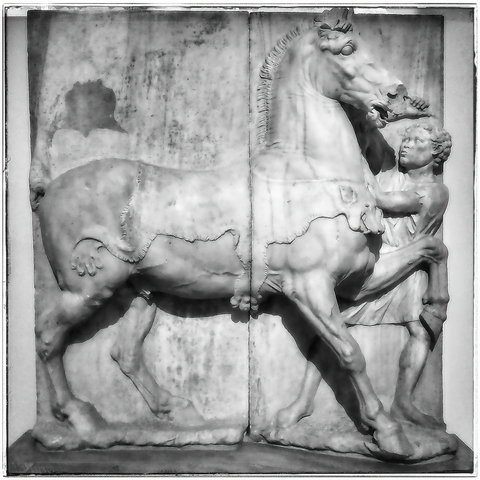
\includegraphics{smallthumb-lesson_I.jpeg}
\setfloatalignment{b}
\end{marginfigure}


\begin{abstract}
\noindent
Queste lezioni si articolano in \textsc{elementi grammaticali}, 
espressi sommariamente, seguiti da \textsc{vocabolari} per il lessico di base 
e da \textsc{frasi da tradurre} dal greco e in greco. 
\
L'approccio è quello del testo-laboratorio di morfosintassi: 
si presenta punto per punto - riprendendone la numerazione - 
l'esposizione di Gleason\cite{gleason1903}.\\
\bigskip
\noindent
Lezione VII: la declinazione in A (la prima declinazione), nomi femminili in ᾱ o η, aggettivi della Declinazione in vocale, vocabolario, esercizi.
\end{abstract}

%\printclassoptions

\newthought{87.} I nomi femminili di questa declinazione terminano in \textbf{α} o \textbf{η}, quelli maschili in \textbf{ᾱς} o \textbf{ης}.

\newthought{88.} La radice del nome termina in \textbf{α}, che al singolare è spesso allungata in 
\textbf{ᾱ} (dopo \textbf{ε, ι} o \textbf{ρ}) o \textbf{η.}

I nomi femminili di questa declinazione terminano in \textbf{ᾱ} o \textbf{η}, quelli maschili in \textbf{ᾱς} o \textbf{ης}.

\newthought{89. Modelli}

\begin{fullwidth}
\begin{table}[!htbp]
  \centering
  \begin{tabular}{l l c l l l l}
    %\toprule
	\multicolumn{7}{c}{\textsc{parole guida}} \\
	\multicolumn{2}{c}{\textbf{ὥρᾱ,}}              & \textsc{nome latino}    & \textbf{ἄκρᾱ,}  & \multicolumn{3}{c}{\textbf{ἡ μῑκρὰ σκηνή,}} \\
	\multicolumn{2}{c}{\textit{tempo, ora,} \textsc{F.}} & \textsc{corrispondente} & \textit{cittadella,} \textsc{f.}  & \multicolumn{3}{c}{\textit{la piccola tenda}} \\
   
	\multicolumn{7}{c}{\textsc{singolare}} \\
    \textsc{n.} & \textbf{ὥρᾱ} & \textit{hōra} & \textbf{ἄκρᾱ} & \textbf{ἡ}   & \textbf{μῑκρὰ} & \textbf{σκηνή}  \\
    \textsc{g.} & \textbf{ὥρᾱς} & \textit{hōrae}  & \textbf{ἄκρᾱς} & \textbf{τῆς} & \textbf{μῑκρᾶς} & \textbf{σκηνῆς}  \\
    \textsc{d.} & \textbf{ὥρᾳ}  & \textit{hōrae}  & \textbf{ἄκρᾳ}  & \textbf{τῇ}  & \textbf{μῑκρᾷ}  & \textbf{σκηνῇ}  \\
	\textsc{a.} & \textbf{ὥρᾱν} & \textit{hōram} & \textbf{ἄκρᾱν} & \textbf{τὴν} & \textbf{μῑκρὰν} & \textbf{σκηνήν}  \\
	\textsc{v.} & \textbf{ὥρᾱ}  & \textit{hōra}  & \textbf{ἄκρᾱ}  & \textemdash  & \textbf{μῑκρὰ}  & \textbf{σκηνή}  \\
	
	\multicolumn{7}{c}{\textsc{plurale}} \\
	\textsc{n.v.} & \textbf{ὧραι}  & \textit{hōrae}    & \textbf{ἄκραι}  & \textbf{αἱ}   & \textbf{μῑκραὶ}  & \textbf{σκηναί}  \\
    \textsc{g.} & \textbf{ὡρῶν}  & \textit{hōrārum} & \textbf{ἄκρῶν}  & \textbf{τῶν}  & \textbf{μῑκρῶν}  & \textbf{σκηνῶν}  \\
    \textsc{d.} & \textbf{ὥραις} & \textit{hōrīs}   & \textbf{ἄκραις} & \textbf{ταῖς} & \textbf{μῑκραῖς} & \textbf{σκηναῖς}  \\
	\textsc{a.} & \textbf{ὥρᾱς} & \textit{hōrās}   & \textbf{ἄκρᾱς} & \textbf{τὰς} & \textbf{μῑκρὰς} & \textbf{σκηνάς}  \\
    %\bottomrule
  \end{tabular}
  \label{tab:normaltab}
  %\zsavepos{pos:normaltab}
\end{table}
\end{fullwidth}

\newpage

\newthought{Osservazione}
\begin{itemize}
\item[\textsc{1.}] In tutte le parole sopra, il genitivo plurale ha l'accento circonflesso sull'ultima sillaba\sidenote{la parola in questo caso si dice \textit{perispomena}.}. Questo accade perché la sillaba risulta da una contrazione di \textbf{-άων}, e vale per tutti i nomi della Declinazione in A. 
\end{itemize}


\newthought{90. Aggettivi e concordanza} La maggior parte degli aggettivi in Greco vengono declinati e, come in latino, concordano in caso, genere e numero con il nome cui si riferiscono\sidenote{o limitano, nel senso che l'aggettovo precisa il senso del nome limitandolo opportunamente: un vaso rosso non può essere di un altro colore.}.

\newthought{91.} Gli aggettivi della Declinazione in vocale\sidenote{\textit{Declinazione in Vocale:} indica sia la Declinazione in O che la Declinazione in A.} si declinano al maschile e al neutro come i nomi (della Declinazione in O) in \textbf{-ος} e \textbf{-ον}, al femminile come i nomi (della Declinazione in A) in \textbf{ᾱ} o \textbf{η.}
Quindi avremo: \nom \textbf{ἀγαθός, ἀγαθή, ἀγαθόν} \gen \textbf{ἀγαθοῦ, ἀγαθῆς, ἀγαθοῦ,} ecc.\sidenote{Cfr. in Latino \textit{bonus, bona, bonum}}

\newthought{Aggettivi della Declinazione in Vocale.}(681, anticipazione)

\begin{fullwidth}
\begin{table}[!htbp]
  \centering
  \begin{tabular}{l l l l l l l l}
    %\toprule
	\multicolumn{8}{c}{\textsc{parole guida}} \\
	& \multicolumn{3}{c}{\textbf{ἀγαθός,} \textit{buono}} & \quad & \multicolumn{3}{c}{\textbf{φίλιος,} \textit{amichevole}} \\
	\multicolumn{8}{c}{\textsc{singolare}} \\
	& \multicolumn{1}{c}{\textsc{masc}} & \multicolumn{1}{c}{\textsc{femm}} & \multicolumn{1}{c}{\textsc{neut}} & \quad & \multicolumn{1}{c}{\textsc{masc}} & \multicolumn{1}{c}{\textsc{femm}} & \multicolumn{1}{c}{\textsc{neut}} \\
    \textsc{n.} & \textbf{ἀγαθός} & \textbf{ἀγαθή} & \textbf{ἀγαθόν} & \quad   & \textbf{φίλιος} & \textbf{φιλία} & \textbf{φίλιον}  \\
    \textsc{g.} & \textbf{ἀγαθοῦ} & \textbf{ἀγαθῆς} & \textbf{ἀγαθοῦ} & \quad   & \textbf{φίλιου} & \textbf{φιλίας} & \textbf{φίλιου}  \\
	\textsc{d.} & \textbf{ἀγαθῷ} & \textbf{ἀγαθῇ} & \textbf{ἀγαθῷ} & \quad   & \textbf{φίλιῳ} & \textbf{φίλιᾳ} & \textbf{φίλιῳ}  \\
	\textsc{a.} & \textbf{ἀγαθόν} & \textbf{ἀγαθήν} & \textbf{ἀγαθόν} & \quad   & \textbf{φίλιος} & \textbf{φίλιος} & \textbf{φίλιος}  \\
	\textsc{v.} & \textbf{ἀγαθέ} & \textbf{ἀγαθή} & \textbf{ἀγαθόν} & \quad   & \textbf{φίλιε} & \textbf{φιλία} & \textbf{φίλιον}  \\
	
	\multicolumn{8}{c}{\textsc{plurale}} \\
	& \multicolumn{1}{c}{\textsc{masc}} & \multicolumn{1}{c}{\textsc{femm}} & \multicolumn{1}{c}{\textsc{neut}} & \quad & \multicolumn{1}{c}{\textsc{masc}} & \multicolumn{1}{c}{\textsc{femm}} & \multicolumn{1}{c}{\textsc{neut}} \\
	\textsc{n.v.} & \textbf{ἀγαθοί} & \textbf{ἀγαθαί} & \textbf{ἀγαθά} & \quad   & \textbf{φίλιοι} & \textbf{φίλιαι} & \textbf{φίλια}  \\
    \textsc{g.} & \textbf{ἀγαθῶν} &\textbf{ἀγαθῶν} & \textbf{ἀγαθῶν} & \quad   & \textbf{φιλίων} & \textbf{φιλίων} & \textbf{φιλίων}  \\
	\textsc{d.} & \textbf{ἀγαθοῖς} & \textbf{ἀγαθαῖς} & \textbf{ἀγαθοῖς} & \quad   & \textbf{φιλίοις} & \textbf{φιλίαις} & \textbf{φιλίοις}  \\
	\textsc{a.} & \textbf{ἀγαθούς} & \textbf{ἀγαθάς} & \textbf{ἀγαθός} & \quad   & \textbf{φιλίοις} & \textbf{φιλίας} & \textbf{φίλια}  \\
	
    %\bottomrule
  \end{tabular}
  \label{tab:normaltab}
  %\zsavepos{pos:normaltab}
\end{table}
\end{fullwidth}

\newthought{Osservazione}
\begin{itemize}
\item[\textsc{1.}] Alcuni aggettivi \textit{(a due uscite)}, seguono la sola Declinazione in O: il maschile e il femminile si declinano allo stesso modo. 
\end{itemize}

\newthought{92. Esercizi}
\begin{itemize}
\item[\textsc{1.}] Declina in tutti i generi \textbf{καλός, σοφός, κακός, δίκαιος.}
\item[\textsc{2.}] Scrivi la declinazione di \textit{la valida barca, la terribile battaglia.}
\end{itemize}

\newpage

\newthought{93. Vocabolario}

\begin{multicols}{2}
    \noindent \hangindent=1em \textbf{ἄκρᾱ,} \textit{altura, cittadella}.  \\
    \noindent \hangindent=1em \textbf{ἐπιστολή,} \textit{lettera}.  \\
    \noindent \hangindent=1em \textbf{ἡμέρᾱ,} \textit{giorno}.  \\
    \noindent \hangindent=1em \textbf{κώμη,} \textit{villaggio}.  \\
    \noindent \hangindent=1em \textbf{μάχη,} \textit{battaglia}.  \\
    \noindent \hangindent=1em \textbf{οἰκίᾱ,} \textit{casa}.  \\
    \noindent \hangindent=1em \textbf{πόλεμος,} \textit{guerra}.  \\
    \noindent \hangindent=1em \textbf{σκηνή,} \textit{tenda}.  \\
	
    \noindent \hangindent=1em \textbf{χώρᾱ,} \textit{terra, nazione}.  \\
    \noindent \hangindent=1em \textbf{ὥρᾱ,} \textit{ora, stagione, tempo}.  \\
	
	\noindent \hangindent=1em \textbf{δέκα,} agg.indecl. \textit{dieci}. \\ 
	
	
    \noindent \hangindent=1em \textbf{μακρός, ά, όν,} \textit{lungo, grande}.  \\
	\noindent \hangindent=1em \textbf{μικρός, ά, όν,} \textit{corto, piccolo}.  \\
	\noindent \hangindent=1em \textbf{φοβερός, ά, όν,} agg. \textit{spaventevole, terribile}.  \\
\end{multicols}

\newthought{94. Traduci:}
\textsc{1.}~τῆς ἡμέρας. \quad
\textsc{2.}~δέκα σκηναῖς. \quad
\textsc{3.}~μακρᾶς μάχης. \quad
\textsc{4.}~τῶν μικρῶν οἰκιῶν. \quad
\textsc{5.}~αἱ τῆς χώρας κῶμαι.

% ᾷῇῷ
% ᾳῃῳ
\newthought{95. Traduci:}
\textsc{1.}~ὁ τῶν θεῶν πόλεμος ἦν φοβερός. \quad
\textsc{2.}~τὰ γὰρ τέκνα οὐκ εἶχε\sidenote{imperfetto di ἔχω (da ἔεχον).} πλοῖα. \quad
\textsc{3.}~ἐν δὲ τῇ μικρᾷ κώμῃ ἦν μάχη φοβερά. \quad
\textsc{4.}~εἰς γὰρ τὴν οἰκίαν ἔφυγον οἱ δοῦλοι. \quad
\textsc{5.}~καὶ ἐκ τῶν σκηνῶν ἔβαλλον λίθους μακρούς. \quad
\textsc{6.}~ἡμέρᾱς δέκα ἐμένομεν ἐν τῷ ἱερῷ. \quad
\textsc{7.}~ὥρα ἦν πέμπειν\sidenote{presente infinito attivo.} τὰς ἐπιστολάς. \quad
\textsc{8.}~τὰ κακὰ παιδία οὐκ ἔλυσαν τοὺς ἵππους. \quad
\textsc{9.}~τίς γὰρ ἁρπάσει τὰς τῆς ἄκρας οἰκίας; \quad
\textsc{10.}~τί γράφεις; \quad
\textsc{11.}~τί ηὖρες ἐπὶ τῷ ποταμῷ;


\newthought{96.} 
\textbf{Διάλογος.} \textemdash 
\textbf{Δύο}\sidenote{due.}\textbf{Μαθηταί}

\begin{itemize}
\item[Μικρός.] Ὁ ἐμος πατὴρ\sidenote{Cfr. in latino \textit{meus pater}} ἔπεμψέ 
\stackunder{μοι}{\scriptsize{me}} τὴμερον δῶρον καλόν.
\item[Μακρός.] \stackunder{Καλῶς!}{\scriptsize{bello!}} τί ἐστιν;

\item[Μικ.] \stackunder{Οὔποτε}{\scriptsize{giammai}} 
\stackunder{εἰκάζειν}{\scriptsize{indovinare}} 
\stackunder{δυνήσει.}{\scriptsize{potrai}}
\item[Μακ.] Τοῦτ´ \stackunder{οἶδα.}{\scriptsize{Lo so}} 
ἀλλὰ \stackunder{λέγε}{\scriptsize{di'}} 
μοι \stackunder{ὡς τάχιστα,}{\scriptsize{subito,}} 
\stackunder{ὠς}{\scriptsize{come}} παιδίον ἀγαθόν.

\item[Μικ.] \stackunder{Ἰδού,}{\scriptsize{Guarda qui,}} πλοῖον καλόν.
\item[Μακ.] Καλῶς, καλῶς! νῦν γὰρ ὥρα ἐστὶ \stackunder{καταβαίνειν}{\scriptsize{scendere}} ἐπὶ τὸν ποταμόν.

\item[Μικ.] Οὐ δῆτα. τήμερον γὰρ ὁ πατὴρ ἐκέλευσέ με μένειν
ἐν τῇ οἰκίᾳ. ἔπαισα γὰρ τὸν ἐμὸν ἀδελφὸν καὶ ἥρπασα τὸ ἱμάτιον αὐτοῦ\sidenote{suo.}.
\item[Μακ.] \stackunder{Ὡς}{\scriptsize{Come}} φοβερόν! 
ἀλλὰ \stackunder{μὴ φρόντιζε.}{\scriptsize{non importa.}} 
\stackunder{κἀγὼ}{\scriptsize{Anch'io}} ἐν τῇ οἰκίᾳ 
μενῶ\sidenote{futuro indicativo.} καὶ ἐπιστολὴν μακρὰν γράψω τῷ ἀδελφῷ.
\end{itemize}

\begin{figure*}[!b]
  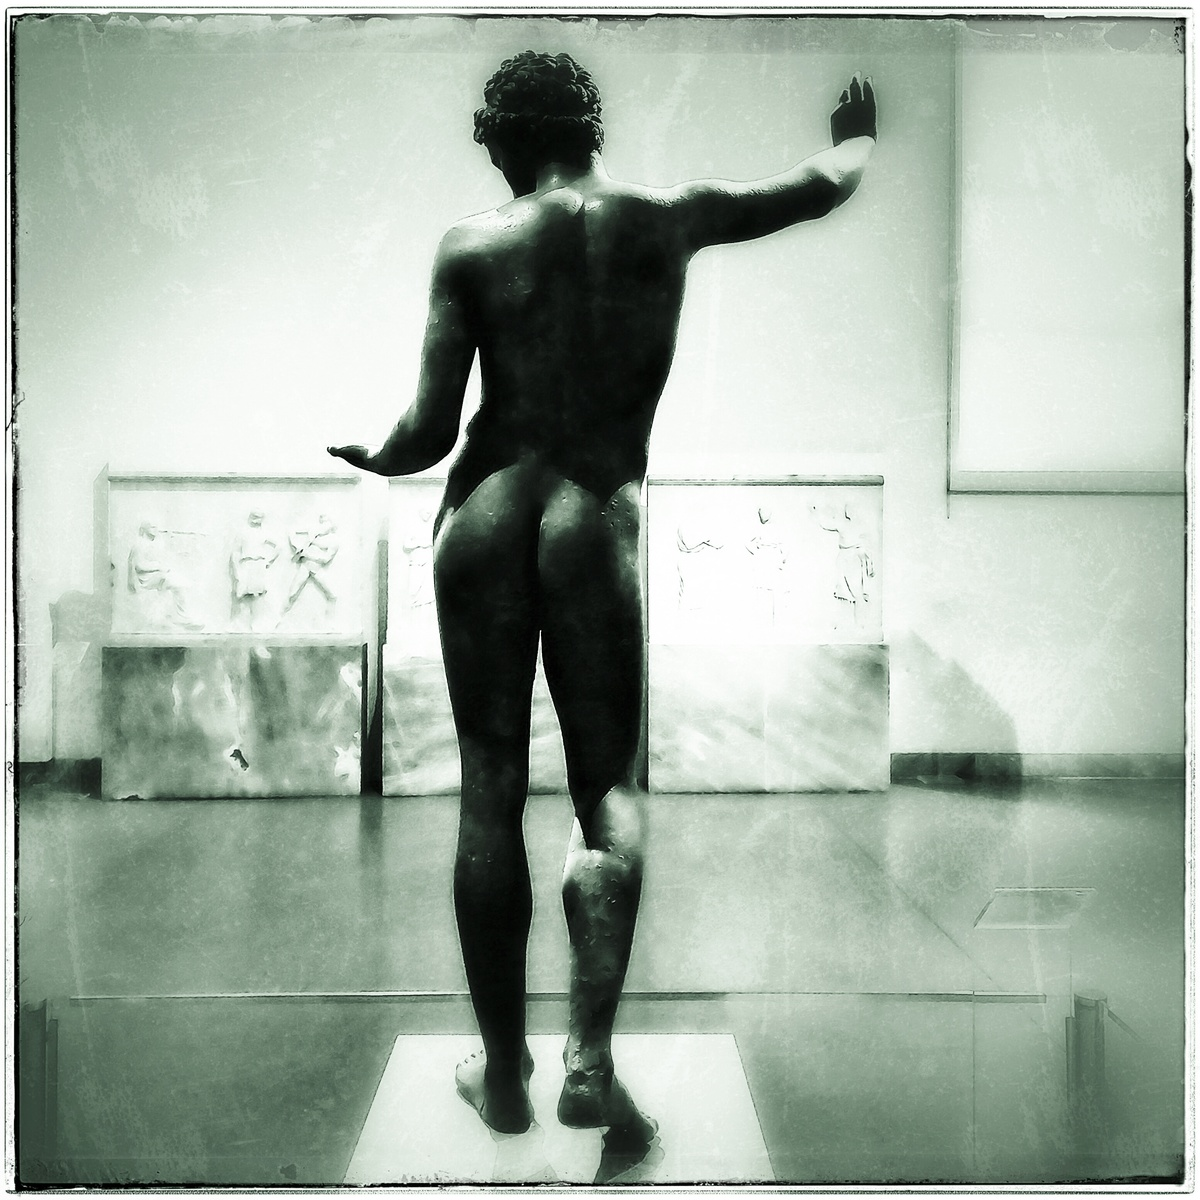
\includegraphics{thumb-lesson_VII.jpeg}
  \caption{Museo Nazionale di Archeologia di Atene}
  \label{fig:textfig}
  %\zsavepos{pos:textfig}
  %\setfloatalignment{b}
\end{figure*}

 

\nobibliography{greekBiblio}
\bibliographystyle{alpha}


\end{document}
